\chapter{Background & State of the Art} \label{chap:sota}

\section*{}

This chapter has two purposes: describing the foundations on which this work
is built on, namely Machine Learning (ML), Probabilistic Reasoning (PR),
Prograbilistic Programming (PP) and
Visual Programming(VP) while enumerating different tools which are based
on one of these concepts.

\subsection{Machine learning}

Machine learning is a field which can be seen as a subfield of artifical
intelligence that incorporates mathematics and statistics and is concerned
with conceiving algorithms that learn autonomously, that is, without human
interventation \cite{mlbrit}\cite{mlnot}.
It has the potential to impact a wide spectrum of
different areas such as biology, medicine, finance, astronomy
\cite{Amatriain:2013:BDU:2541176.2514691}, computer vision, sales forecast,
robotics \cite{intml}, product recommendations, fraud detection or
internet ads bidding \cite{SciPy}.

Learning from data is commercially and scientifically important. ML consists of
methods that automatically extract interesting knowledge in databases of sometimes chaotic and
redundant information. ML is a data-based knowledge-discovering process that
has the potential not only to analyze events in retrospect but also to predict
future events or important alterations \cite{mapt}.

\subsection{Probabilistic Reasoning}

Probabilistic reasoning is the formation of probability judgments and of
subjective beliefs about the likelihoods of outcomes and the frequencies of
events \cite{probr}, it is a way to combine our knowledge of a situation
with the laws of probability. There are subjective belifs because, in non-trivial
decision-making there are unobserved factors that are critical to the decision
in conjunction with several sources of uncertainty \cite{reas}, such as:

\begin{itemize}
  \item Uncertain inputs, due to missing or noisy data
  \item Uncertain knowledge, where multiple causes lead to multiple effects,
  or there is an incomplete knowledge of conditions, effects and causality of the
  domain or simply because the effects are inherently stochastic.
\end{itemize}

So, probabilistic reasoning only gives probabilistic results.

It is one way to
overcome cognitive bias and be able to make rational decisions \cite{Sedlmeier2001}.
A trial has been made \cite{christensen1982experience}
where physicians were asked to estimate the probability that a
woman with a positive mammogram actually has breast cancer, given a base rate of
1\% for breast cancer, a hit rate of about 80\%, and a false-alarm rate of about
10\%. It reported that 95 of 100 physicians estimated the probability that she
actually has breast cancer to be between 70\% and 80\%, whereas Bayes's rule
gives a value of about 7.5\%. Such systematic deviations from Bayesian reasoning
have been called "cognitive illusions,". We will describe both Bayes's rules
and Bayesian reasoning in the next section.

\subsubsection{Bayesian Reasoning}

One way to approach PR is by using bayesian reasoning, which is inspired in the
Bayes Theorem. An equivalent rule to the theorem, in its simplest form (applied
to a single event) is:

$$ P(A \mid B) = \frac{P(A \land B)}{P(B)} $$

Where P(A|B) defines the probability of event A given that B occurred.
The theorem defines how hidden causes (A) relate to observed events (B), given
a causality model (P(A, B) or P(B|A)*P(A)) and our knowledge of the probability of the
occurrence of events (P(B)). The inverse is also true, as we will see further
ahead in this section.
As an example, P(penalty | goal) defines the probability that a penalty kick was
scored, knowing that there was a goal.

There are at least two interpretations to the theorem and regarding how one may think
about its results \cite{Fienberg2006}:

\begin{itemize}
  \item Frequentist interpreation: probabilities are defined by the relative
frequency of events, given a natural sampling. Meaning, the probabiltiy of
obtaining 'Heads' when rolling a dice is equal to the number of 'Heads' obtained
after rolling the dice a sufficient number of times relative to the total number
of times the dice has been rolled.
  \item Epistemological interpreation: probabilities represent a measure of
belief. It can either be a result logical combination of probabilities through
the usage of axioms (it's closely related to Aristotlean logic)
or it can also reflect a personal belief (which is called a subjective view).
\end{itemize}

One example of the application of this theorem is \cite{reas}: you know your home's alarm
is ringing, but you don't know whether that was caused by a burglar or
something else (maybe a bird triggered it, or there was a malfunction in the
alarm system). How confident are you that you're being robbed? Consider that
the alarm company, based on quality trials, defined in the confusion
matrix for P(alarm, burglary) (Table \ref{tab:bayes}).

\begin{table}[t]
  \centering
  \caption{Alarm system confusion matrix}
\begin{tabular}{| l | l | l |}
	\hline
  & alarm & \neg alarm \\ \hline
 burglary & 0.09 & 0.01 \\ \hline
 \neg burglary & 0.1 & 0.8 \\ \hline
\end{tabular}
  \label{tab:bayes}
\end{table}

You can interpret each table's cell as P(A, B). For instances, the top left
cell is the probability that the alarm rings and there is a burglar, while the
bottom left cell is the probability that the alarm rang but there was no burglar
(a false positive).

If we substitute the values of Bayes' rule described above, we get:

$$ P(burglar \mid alarm) = \frac{P(burglar, alarm)}{P(alarm)} $$

Where results is 0.09 / 0.19 = 0.47. So, even if the alarm is ringing, there is
just a 47\% probability that the house is actually being robbed.

The previous example illustrates the simplest case of applied BR, but it is
also possible to combine several variables.
One way to represent this kind of scenario is by expressing the variables in a directed acyclic
graph, where the relation "Parent" stands for "May cause" and you can specify
the conditional probabilities of a child given a parent's result. This graphical
model is called a Bayesian Network.

We can extended our alarm example further, by considering not only a burglar
can trigger the alarm, but an earthquake also can (while there can still be
false positives). Also, consider that we have 2 neighbors (Mary and John) who
may call us whether the alarm is ringing or not. This problem is represented in
figure \ref{beliefnet}.

\begin{figure}[t]
  \begin{center}
    \leavevmode
    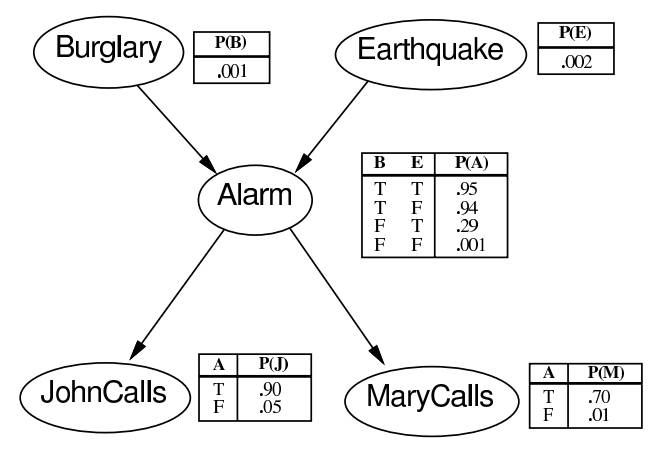
\includegraphics[width=0.86\textwidth]{beliefnet}
    \caption{Belief network for the alarm problem \cite{belfn}}
    \label{fig:beliefnet}
  \end{center}
\end{figure}

Some interesting question we can ask, given this scenario are:

\begin{itemsize}
  \item If John calls saying the alarm is ringing but Mary doesn't, what are the
odds it really is ringing?
  \item If the alarm is ringing, was there an earthquake?
  \item What are the chances that both my neighbors call, the alarm is ringing,
but there is neither a burglary nor an earthquake?
\end{itemize}

This last example, for instances, would be calculated as: P(J, M, A, \neg B, \neg E)
= P(J|A) * P(M|A) * P(A|\neg B, \neg E) * P(\neg B) * P(\neg E) =
0.9 * 0.7 * 0.001 * 0.999 * 0.998 = 0.00062. Notice how counter-intuitive this
example is: the probability of there being an earthquake is about 32 times larger
then there being an earthquake, the alarm ringing and the neighbors calling us,
even if the conditional probabilities are reasonably high (0.95, 0.9 and 0.7).
This is the result of the calculation of the joint probability being an highly
combinatorial problem, which is yet another argument in favor of using PR
rather than subjective heuristics.

In practical ML applications, it is often the case that there is an
incoming stream of new data, rather than one-time batch calculations.
BR can accomodate this way of thinking, which A. Downey called diachronic
interpretation \cite{thbay}, where diachronic means that something is happening
over time (in this case the probability of the hypotheses, as new data arrives).
In order to make sense of this definition, we may rewrite Bayes' rule as:

$$ P(H \mid D) = \frac{P(D \mid H) \, P(H)}{P(D)} $$

Where:

\begin{itemize}
  \item H: hypothesis
  \item D: data
  \item p(H): probability of the hypothesis before the new data is taken into
account. Also called \textbf{prior}. It can either be calculated using background
information or subjectively defined using domain knowledge. Loses significance
as new data is added, so its choice is not determinant to the model's performance
in the long run.
  \item p(H|D): what we want to calculate, the probability of the hypothesis
after considering the new date. It is called \textbf{posterior}.
  \item p(D|H): probability of the data if the hypothesis was true, called
the \textbf{likelihood}.
  \item p(D): probability of the data under any hypothesis, called the
\textbf{normalizing constant}.
\end{itemize}

Under this interpretation, you may continuously feed data into the model and see
the probabilities getting updated. We will see more practical examples of this
in section \ref{pp}.

At first glance, someone who is learning for the first time about PR applied
to ML, may think that graphical models such as the one presented in Figure
\ref{beliefnet} are the best there can be done in terms of using a graphical
interface for solving this kind of problems and that the only thing is missing
is an automated way to make the calculations.

While it is true we have never refered mentioned techniques or tools that
automatically do inference over a Bayesian Network, there are several tools
with that capability (including an R package \cite{Højsgaard2013} or
standalone tools \cite{msbn}).

However, not all PR can be done via Bayesian Networks and not all models are graphical
models \cite{intpp}. PP are the largest class of models available, and here are
also more algorithms for inference than just the calculation of joint
probabilities (like we did in the alarm example), as we will discuss in Section
\ref{sec:pp}.

Bayesian Networks are not the only kind of graphical model, another one is
Markov Chains, which is yet another example of a model which is not able to
represent all PR problems. This is clear when we realize that, while PPLs
support a large number of different distributions (such as Normal, Laplace,
Gamma, Half-Cauchy or \textit{t}), all Bayesian Networks and Markov Chain
can be represented in a PPL by just using Bernoulli distributions \cite{PPm}.
We can see an example of such a translation in Figure \ref{fig:mppl}.

\begin{figure}[t]
  \begin{center}
    \leavevmode
    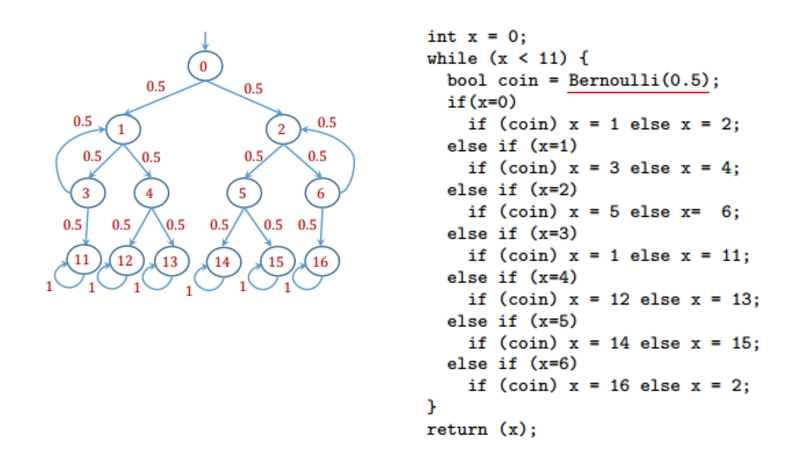
\includegraphics[width=0.86\textwidth]{markppl}
    \caption{Translation of Discrete Time Markov Chain to a PPL \cite{PPm}}
    \label{fig:mppl}
  \end{center}
\end{figure}

\subsubsection{Probabilistic Programming Languages}
\label{sec:pp}

Until recently, probabilistic reasoning systems have been limited in scope, and
have been hard to apply to many real world situations. Models are communicated
using a mix of natural language, pseudo code, and mathematical formulae and solved
using special purpose, one-off inference methods. Rather than precise
specifications suitable for automatic inference, graphical models typically
serve as coarse, high-level descriptions, eliding critical aspects such as
fine-grained independence, abstraction and recursion.

Probabilistic programming is a new approach that makes probabilistic reasoning
systems easier to build and more widely applicable. A probabilistic programming
language (PPL) is a programming language designed to describe probabilistic
models, in a such a way we can say that the program itself is the model, and
then perform inference in those models. PPLs have seen recent interest from the
artificial intelligence, programming languages, cognitive science, and natural
languages communities. By empowering users with a common dialect in the form of
a programming language, rather than requiring each one of them to the
non-trivial and error-prone task of writing their own models and hand-tailored
inference algorithms for the problem at hand, it encourages exploration, since
different models require less time to setup and evaluate, and enables sharing
knowledge in the form of best practices, patterns and tools such as optimized
compilers or interpreters, debuggers, IDE’s, optimizers and profilers.

Algoritmos
PPLs are closely related to graphical models and Bayesian networks, but are more
expressive and flexible. One can easily realize this by looking at the re-usable
components PPLs offer, being one of them the inference engine, which can be
plugged in into different models. For instances, it is easy to replace the
exact-solution traditional Bayesian networks inference, which requires time
exponential in the number of variables to run, with approximation algorithms
such as the Markov Chain Monte Carlo (MCMC) or Variational Message Passing
(VMP), which make it possible to compute large hierarchical models by resorting
to sampling and approximation. 

Mais custom que ML, exemplo truskill

When compared to other machine learning methods (such as random forests, neural
networks or linear regression), which take homogeneous data as input (requiring
the user to separate their domain into different models), probabilistic
programming is used to leverage the data’s original structure.

\begin{quote}
  ``If we view the semantics of the underlying deterministic language as a map
  from programs to executions of the program, the semantics of a PPL built on it
   will be a map from programs to distributions over executions. When the
   program halts with probability one, this induces a proper distribution over
   return values. Indeed, any computable distribution can be represented as the
   distribution induced by a Church program in this way''~\cite{Freer2012}
\end{quote}

Distributions e nao so prob, exemplo dos slides com graficos

Plus, it provides full probability distributions over both the predictions and parameters of the
model, whereas ML methods can only give the user a certain degree of confidence
on the predictions.

\subsection{Visual Programming}

\subsubsection{Visual Dataflow Programming}

\subsection{State of the Art}

PPLs often extend from a basic language (i.e.,
they are embedded in a host language like R, Java or Scala), although some PPLs
such as WinBUGS and Stan offer a self-contained language, with no obvious origin
in another language.

\subsubsection{Stan}

\subsubsection{WinBUGS}

\subsubsection{Church}

\subsubsection{Infer.NET}

\subsubsection{PyMC}

\subsubsection{VIBES}

\subsubsection{NoFlo}

\subsubsection{RapidMiner}

\subsubsection{Weka Knowledge FLow}

\subsubsection{GoJS}

\subsubsection{Blockly}

\subsubsection{Viskell}

\section{Conclusions}
